% -*-latex-*-
% 
% For questions, comments, concerns or complaints:
% thesis@mit.edu
% 
%
% $Log: cover.tex,v $
% Revision 1.8  2008/05/13 15:02:15  jdreed
% Degree month is June, not May.  Added note about prevdegrees.
% Arthur Smith's title updated
%
% Revision 1.7  2001/02/08 18:53:16  boojum
% changed some \newpages to \cleardoublepages
%
% Revision 1.6  1999/10/21 14:49:31  boojum
% changed comment referring to documentstyle
%
% Revision 1.5  1999/10/21 14:39:04  boojum
% *** empty log message ***
%
% Revision 1.4  1997/04/18  17:54:10  othomas
% added page numbers on abstract and cover, and made 1 abstract
% page the default rather than 2.  (anne hunter tells me this
% is the new institute standard.)
%
% Revision 1.4  1997/04/18  17:54:10  othomas
% added page numbers on abstract and cover, and made 1 abstract
% page the default rather than 2.  (anne hunter tells me this
% is the new institute standard.)
%
% Revision 1.3  93/05/17  17:06:29  starflt
% Added acknowledgements section (suggested by tompalka)
% 
% Revision 1.2  92/04/22  13:13:13  epeisach
% Fixes for 1991 course 6 requirements
% Phrase "and to grant others the right to do so" has been added to 
% permission clause
% Second copy of abstract is not counted as separate pages so numbering works
% out
% 
% Revision 1.1  92/04/22  13:08:20  epeisach

% NOTE:
% These templates make an effort to conform to the MIT Thesis specifications,
% however the specifications can change.  We recommend that you verify the
% layout of your title page with your thesis advisor and/or the MIT 
% Libraries before printing your final copy.
%\department{Faculty of Electronics and Information Technology}


\title{Sensor data acquisition for scientific grade cameras}

%
%\author{Piotr Zdunek}
%\indexnumber{229417}
%\specialty{Microsystems and Electronic Systems}
%\field{Electronics}
%\type{Master Thesis}
%\institute{Institute of Electronic Systems}
%\supervisor{Grzegorz Kasprowicz, PhD}
%\city{Warsaw}
%\degreemonth{Feburary}
%\degreeyear{2017}

% If you wish to list your previous degrees on the cover page, use the 
% previous degrees command:
%       \prevdegrees{A.A., Harvard University (1985)}
% You can use the \\ command to list multiple previous degrees
%       \prevdegrees{B.S., University of California (1978) \\
%                    S.M., Massachusetts Institute of Technology (1981)}

% If the thesis is for two degrees simultaneously, list them both
% separated by \and like this:
% \degree{Doctor of Philosophy \and Master of Science}

% As of the 2007-08 academic year, valid degree months are September, 
% February, or June.  The default is June.
%\thesisdate{20.09.2016}

%% By default, the thesis will be copyrighted to MIT.  If you need to copyright
%% the thesis to yourself, just specify the `vi' documentclass option.  If for
%% some reason you want to exactly specify the copyright notice text, you can
%% use the \copyrightnoticetext command.  
%\copyrightnoticetext{\copyright Warsaw University of Technology}

% If there is more than one supervisor, use the \supervisor command
% once for each.

% Make the titlepage based on the above information.  If you need
% something special and can't use the standard form, you can specify
% the exact text of the titlepage yourself.  Put it in a titlepage
% environment and leave blank lines where you want vertical space.
% The spaces will be adjusted to fill the entire page.  The dotted
% lines for the signatures are made with the \signature command.
%\maketitle

% The abstractpage environment sets up everything on the page except
% the text itself.  The title and other header material are put at the
% top of the page, and the supervisors are listed at the bottom.  A
% new page is begun both before and after.  Of course, an abstract may
% be more than one page itself.  If you need more control over the
% format of the page, you can use the abstract environment, which puts
% the word "Abstract" at the beginning and single spaces its text.

%% You can either \input (*not* \include) your abstract file, or you can put
%% the text of the abstract directly between the \begin{abstractpage} and
%% \end{abstractpage} commands.

\cleardoublepage
\includepdf[pages=-]{./chap/titlepage_v4.pdf}
\pagestyle{empty}
\setcounter{savepage}{\thepage}
% First copy: start a new page, and save the page number.
\cleardoublepage
% Uncomment the next line if you do NOT want a page number on your
% abstract and acknowledgments pages.
%\pagestyle{empty}
%\setcounter{savepage}{\thepage}
%
%\begin{abstractpage}
%% $Log: abstract.tex,v $
% Revision 1.0  11.2015 % 
% 
%
%% The text of your abstract and nothing else (other than comments) goes here.
%% It will be single-spaced and the rest of the text that is supposed to go on
%% the abstract page will be generated by the abstractpage environment.  This
%% file should be \input (not \include 'd) from cover.tex.

%Original text:
%In this thesis, I designed and implemented a compiler which performs
%optimizations that reduce the number of low-level floating point operations
%necessary for a specific task; this involves the optimization of chains of
%floating point operations as well as the implementation of a ``fixed'' point
%data type that allows some floating point operations to simulated with integer
%arithmetic.  The source language of the compiler is a subset of C, and the
%destination language is assembly language for a micro-floating point CPU.  An
%instruction-level simulator of the CPU was written to allow testing of the
%code.  A series of test pieces of codes was compiled, both with and without
%optimization, to determine how effective these optimizations were.


In this Master Thesis a Scientific Camera framework design is presented. As far as an embedded system design is
concerned, scientific cameras present a great engineering effort in order to succesfully design and implement this kind
of device. This is why this framework was created, so that an engineer wanting to quickly test his or her design can
benefit from it. Proposed framework is build using Xilinx Zynq SoC and thus allows for creating a camera that has 
a multigigabit data acquisition capability as well as multigigabit transmission using SATA or 10 GbE interfaces. 
What is more, a designer can benefit from using a heterogenous operating system where on a multicore processor 
one core is running a real-time operating system whereas on the second core an embedded Linux operating system is 
being run. This provides a great deal of possibilites for numerous applications. Another feature of the framework is 
the multichannel support where multiple cameras can be synchronised using either a dedicated MLVDS interface or 
Ethernet based Precision-Time-Protocol. Mentioned features given as a tested and ready to use subsusystems of a Xilinx 
Vivado project allows for quicker and less error prone scientific camera design. Project is targeted specifically 
towards scientific camera systems due to the fact that this market is very broad and every project has different
requirements. What is common in all scientific camera projects is the sensor data acquisition, synchronisation
capability as well as data transmission. This proves that such a framework can greatly speed up the development 
of a scientific camera. 

%\end{abstractpage}

\cleardoublepage
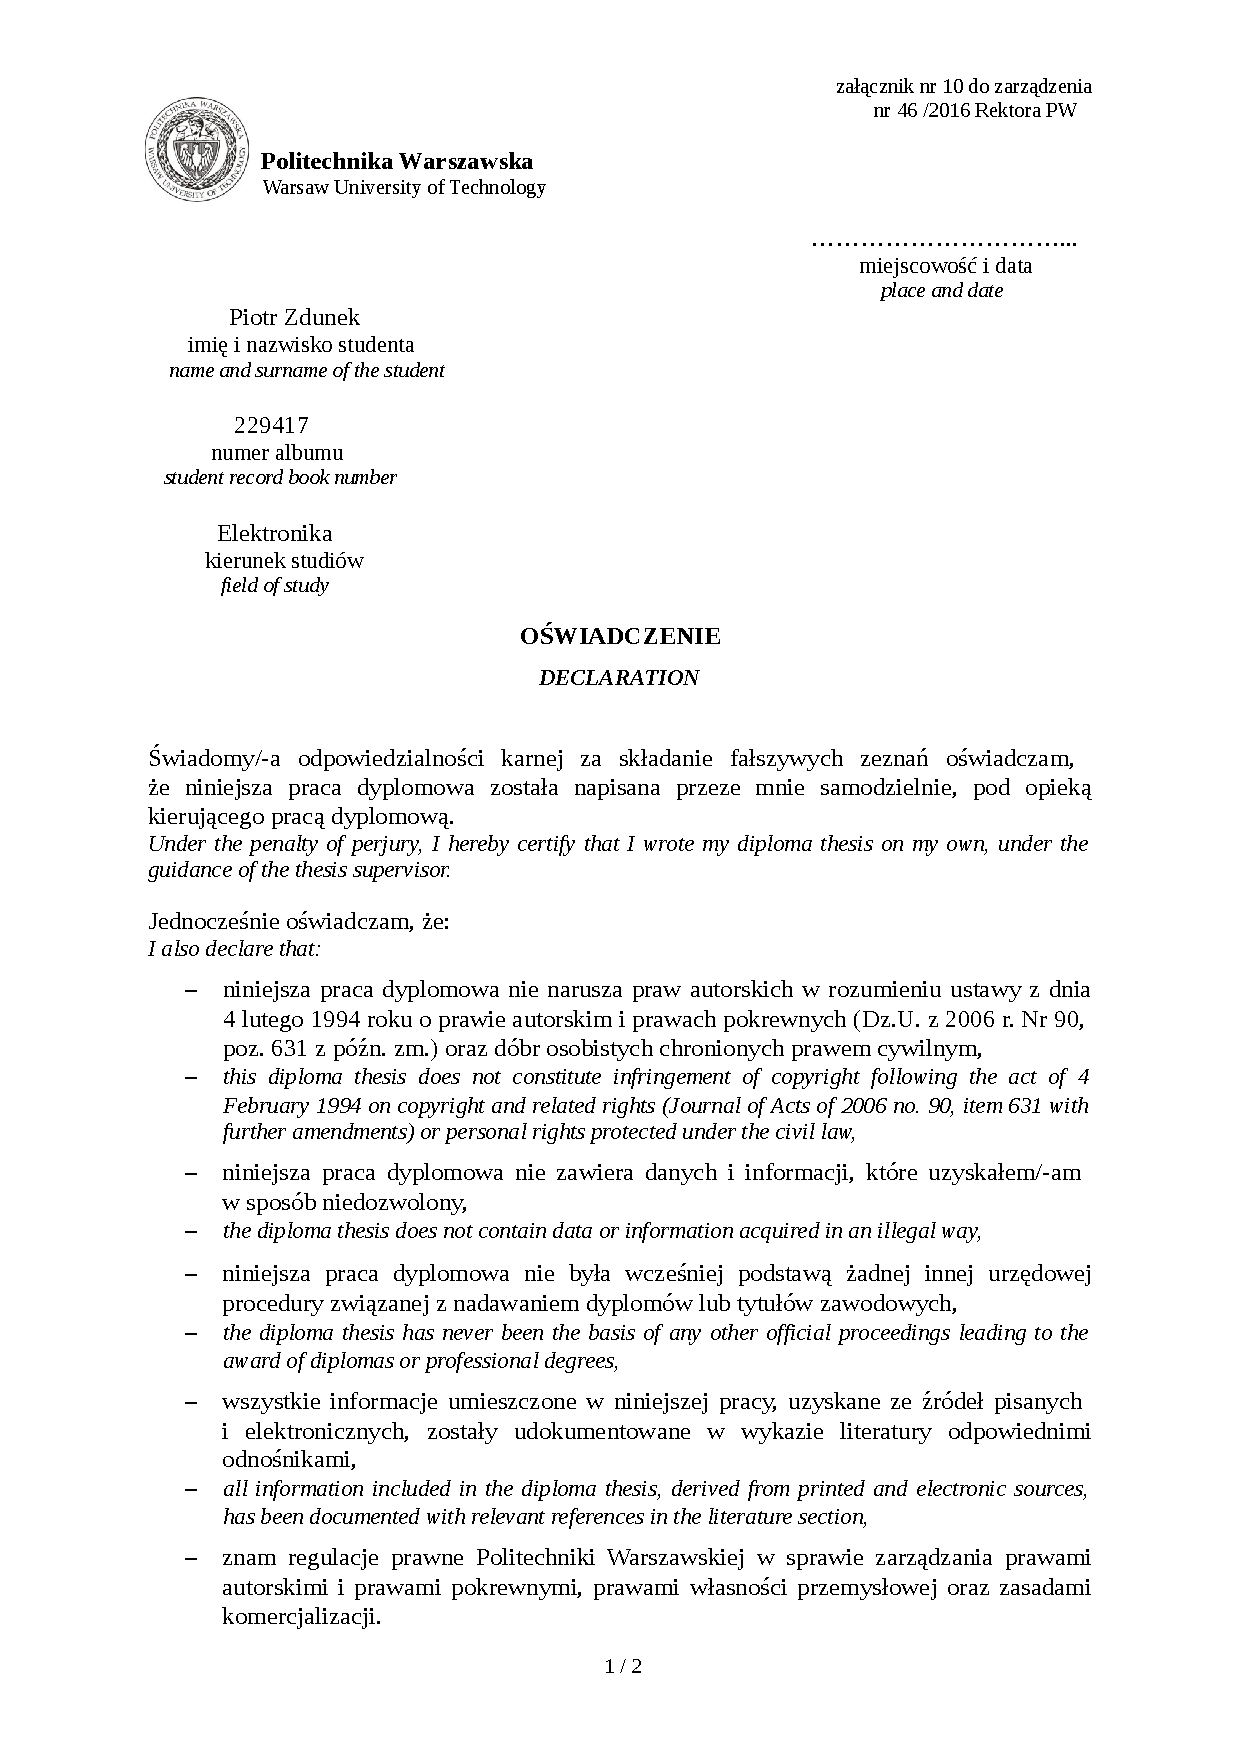
\includepdf[pages=-]{./chap/osw.pdf}
\pagestyle{empty}
\setcounter{savepage}{\thepage}
% First copy: start a new page, and save the page number.
%

\cleardoublepage\null
%
%\begin{abstractpage}
%% $Log: abstract.tex,v $
% Revision 1.0  11.2015 % 
% 
%
%% The text of your abstract and nothing else (other than comments) goes here.
%% It will be single-spaced and the rest of the text that is supposed to go on
%% the abstract page will be generated by the abstractpage environment.  This
%% file should be \input (not \include 'd) from cover.tex.

%Original text:
%In this thesis, I designed and implemented a compiler which performs
%optimizations that reduce the number of low-level floating point operations
%necessary for a specific task; this involves the optimization of chains of
%floating point operations as well as the implementation of a ``fixed'' point
%data type that allows some floating point operations to simulated with integer
%arithmetic.  The source language of the compiler is a subset of C, and the
%destination language is assembly language for a micro-floating point CPU.  An
%instruction-level simulator of the CPU was written to allow testing of the
%code.  A series of test pieces of codes was compiled, both with and without
%optimization, to determine how effective these optimizations were.


In this Master Thesis a Scientific Camera framework design is presented. As far as an embedded system design is
concerned, scientific cameras present a great engineering effort in order to succesfully design and implement this kind
of device. This is why this framework was created, so that an engineer wanting to quickly test his or her design can
benefit from it. Proposed framework is build using Xilinx Zynq SoC and thus allows for creating a camera that has 
a multigigabit data acquisition capability as well as multigigabit transmission using SATA or 10 GbE interfaces. 
What is more, a designer can benefit from using a heterogenous operating system where on a multicore processor 
one core is running a real-time operating system whereas on the second core an embedded Linux operating system is 
being run. This provides a great deal of possibilites for numerous applications. Another feature of the framework is 
the multichannel support where multiple cameras can be synchronised using either a dedicated MLVDS interface or 
Ethernet based Precision-Time-Protocol. Mentioned features given as a tested and ready to use subsusystems of a Xilinx 
Vivado project allows for quicker and less error prone scientific camera design. Project is targeted specifically 
towards scientific camera systems due to the fact that this market is very broad and every project has different
requirements. What is common in all scientific camera projects is the sensor data acquisition, synchronisation
capability as well as data transmission. This proves that such a framework can greatly speed up the development 
of a scientific camera. 

%\end{abstractpage}
%
%
%\begin{abstract}
%% $Log: abstract.tex,v $
% Revision 1.0  11.2015 % 
% 
%
%% The text of your abstract and nothing else (other than comments) goes here.
%% It will be single-spaced and the rest of the text that is supposed to go on
%% the abstract page will be generated by the abstractpage environment.  This
%% file should be \input (not \include 'd) from cover.tex.

%Original text:
%In this thesis, I designed and implemented a compiler which performs
%optimizations that reduce the number of low-level floating point operations
%necessary for a specific task; this involves the optimization of chains of
%floating point operations as well as the implementation of a ``fixed'' point
%data type that allows some floating point operations to simulated with integer
%arithmetic.  The source language of the compiler is a subset of C, and the
%destination language is assembly language for a micro-floating point CPU.  An
%instruction-level simulator of the CPU was written to allow testing of the
%code.  A series of test pieces of codes was compiled, both with and without
%optimization, to determine how effective these optimizations were.


In this Master Thesis a Scientific Camera framework design is presented. As far as an embedded system design is
concerned, scientific cameras present a great engineering effort in order to succesfully design and implement this kind
of device. This is why this framework was created, so that an engineer wanting to quickly test his or her design can
benefit from it. Proposed framework is build using Xilinx Zynq SoC and thus allows for creating a camera that has 
a multigigabit data acquisition capability as well as multigigabit transmission using SATA or 10 GbE interfaces. 
What is more, a designer can benefit from using a heterogenous operating system where on a multicore processor 
one core is running a real-time operating system whereas on the second core an embedded Linux operating system is 
being run. This provides a great deal of possibilites for numerous applications. Another feature of the framework is 
the multichannel support where multiple cameras can be synchronised using either a dedicated MLVDS interface or 
Ethernet based Precision-Time-Protocol. Mentioned features given as a tested and ready to use subsusystems of a Xilinx 
Vivado project allows for quicker and less error prone scientific camera design. Project is targeted specifically 
towards scientific camera systems due to the fact that this market is very broad and every project has different
requirements. What is common in all scientific camera projects is the sensor data acquisition, synchronisation
capability as well as data transmission. This proves that such a framework can greatly speed up the development 
of a scientific camera. 

%\end{abstract}
%
%% First copy: start a new page, and save the page number.
% Uncomment the next line if you do NOT want a page number on your
% abstract and acknowledgments pages.
\cleardoublepage
% Uncomment the next line if you do NOT want a page number on your
% abstract and acknowledgments pages.
\pagestyle{empty}
\setcounter{savepage}{\thepage}

%\begin{abstractpage}
%%\large{\textbf{Tytuł:} System realizacji kamer do zastosowań naukowych.}\\

\thispagestyle{empty}
\setcounter{savepage}{\thepage}

\begin{center}

%\textbf{Title: Camera design framework for scientific applications}
\large{\textbf{Tytuł:} Akwizycja danych z czujników optycznych dla kamer do zastosowań naukowych}

\vspace{0.5cm}
\textbf{Streszczenie}

\end{center}
%
%
%W ramach niniejszej pracy magisterskiej wykonane zostało oprogramowanie na system wbudowany pozwalające na realizację 
%kamer do zastosowań naukowych. Rozwój kamer jest skomplikowanym i długotrwałym procesem. Projekt powstał, aby wspomóc
%tworzenie prototypu takiej kamery. Dzięki niemu możliwe jest szybkie sprawdzenie koncepcji swojej aplikacji 
%wykorzystując gotowe podsystemy.
%
%Aplikacja wykorzystuje Xilinx Zynq SoC dzięki czemu umożliwia realizację urządzenia posiadającego możliwość
%akwizycji znacznej ilości danych oraz możliwość transmisji danych z wielogigabitową przepustowością. 
%
%Dodatkowo system jest wyposażony w heterogeniczny system operacyjny, który pracuje na dwurdzeniowym układzie
%Cortex A9. Na jednym rdzeniu uruchomiony jest system czasu rzeczywistego FreeRTOS, a na drugim system operacyjny
%wysokiego poziomu Linux. Taki tandem pozwala na elastyczną realizację wielu aplikacji. Dodatkowo dzięki wykorzystaniu
%Ethernet system pozwala na pracę wielokanałową z wykorzystaniem standardu synchronizacji czasu
%Precision-Time-Protocol. 
%
%Wspomniane funkcje kamery zrealizowane w formie elastycznego systemu do prototypowania kamer pozwala na szybką realizację 
%prototypu kamery, gdzie podstawowe funkcjonalności są już zaimplementowane. Pozwala to na zmniejszenie ilości błędów oraz 
%sprawdzenie poprawności koncepcji. Mając na uwadze powyższe, projekt zrealizowany w ramach 
%pracy magisterskiej może mieć szerokie zastosowanie zarówno w przemyśle jak i w nauce. 
%
%W pierwszym rozdziale opisane zostały podstawowe informacje dotyczące kamer i uwzględnieniem szczególnych parametrów
%kamer do zastosowań naukowych. Rozdział 2 przedstawia genezę oraz wymagania projektu. Następnie, w rozdziale 3
%zaprezentowana została koncepcja realizacji aplikacji i w rozdziale 4 sama realizacja wraz z wynikami testów. Finalnie,
%rozdział 5 podsumowuje zrealizowany projekt. 
%
\cleardoublepage

%\end{abstractpage}

%\begin{abstractpagepl}
%%\large{\textbf{Tytuł:} System realizacji kamer do zastosowań naukowych.}\\

\thispagestyle{empty}
\setcounter{savepage}{\thepage}

\begin{center}

%\textbf{Title: Camera design framework for scientific applications}
\large{\textbf{Tytuł:} Akwizycja danych z czujników optycznych dla kamer do zastosowań naukowych}

\vspace{0.5cm}
\textbf{Streszczenie}

\end{center}
%
%
%W ramach niniejszej pracy magisterskiej wykonane zostało oprogramowanie na system wbudowany pozwalające na realizację 
%kamer do zastosowań naukowych. Rozwój kamer jest skomplikowanym i długotrwałym procesem. Projekt powstał, aby wspomóc
%tworzenie prototypu takiej kamery. Dzięki niemu możliwe jest szybkie sprawdzenie koncepcji swojej aplikacji 
%wykorzystując gotowe podsystemy.
%
%Aplikacja wykorzystuje Xilinx Zynq SoC dzięki czemu umożliwia realizację urządzenia posiadającego możliwość
%akwizycji znacznej ilości danych oraz możliwość transmisji danych z wielogigabitową przepustowością. 
%
%Dodatkowo system jest wyposażony w heterogeniczny system operacyjny, który pracuje na dwurdzeniowym układzie
%Cortex A9. Na jednym rdzeniu uruchomiony jest system czasu rzeczywistego FreeRTOS, a na drugim system operacyjny
%wysokiego poziomu Linux. Taki tandem pozwala na elastyczną realizację wielu aplikacji. Dodatkowo dzięki wykorzystaniu
%Ethernet system pozwala na pracę wielokanałową z wykorzystaniem standardu synchronizacji czasu
%Precision-Time-Protocol. 
%
%Wspomniane funkcje kamery zrealizowane w formie elastycznego systemu do prototypowania kamer pozwala na szybką realizację 
%prototypu kamery, gdzie podstawowe funkcjonalności są już zaimplementowane. Pozwala to na zmniejszenie ilości błędów oraz 
%sprawdzenie poprawności koncepcji. Mając na uwadze powyższe, projekt zrealizowany w ramach 
%pracy magisterskiej może mieć szerokie zastosowanie zarówno w przemyśle jak i w nauce. 
%
%W pierwszym rozdziale opisane zostały podstawowe informacje dotyczące kamer i uwzględnieniem szczególnych parametrów
%kamer do zastosowań naukowych. Rozdział 2 przedstawia genezę oraz wymagania projektu. Następnie, w rozdziale 3
%zaprezentowana została koncepcja realizacji aplikacji i w rozdziale 4 sama realizacja wraz z wynikami testów. Finalnie,
%rozdział 5 podsumowuje zrealizowany projekt. 
%
\cleardoublepage

%\end{abstractpagepl}

%\begin{abstract}
%%\large{\textbf{Tytuł:} System realizacji kamer do zastosowań naukowych.}\\

\thispagestyle{empty}
\setcounter{savepage}{\thepage}

\begin{center}

%\textbf{Title: Camera design framework for scientific applications}
\large{\textbf{Tytuł:} Akwizycja danych z czujników optycznych dla kamer do zastosowań naukowych}

\vspace{0.5cm}
\textbf{Streszczenie}

\end{center}
%
%
%W ramach niniejszej pracy magisterskiej wykonane zostało oprogramowanie na system wbudowany pozwalające na realizację 
%kamer do zastosowań naukowych. Rozwój kamer jest skomplikowanym i długotrwałym procesem. Projekt powstał, aby wspomóc
%tworzenie prototypu takiej kamery. Dzięki niemu możliwe jest szybkie sprawdzenie koncepcji swojej aplikacji 
%wykorzystując gotowe podsystemy.
%
%Aplikacja wykorzystuje Xilinx Zynq SoC dzięki czemu umożliwia realizację urządzenia posiadającego możliwość
%akwizycji znacznej ilości danych oraz możliwość transmisji danych z wielogigabitową przepustowością. 
%
%Dodatkowo system jest wyposażony w heterogeniczny system operacyjny, który pracuje na dwurdzeniowym układzie
%Cortex A9. Na jednym rdzeniu uruchomiony jest system czasu rzeczywistego FreeRTOS, a na drugim system operacyjny
%wysokiego poziomu Linux. Taki tandem pozwala na elastyczną realizację wielu aplikacji. Dodatkowo dzięki wykorzystaniu
%Ethernet system pozwala na pracę wielokanałową z wykorzystaniem standardu synchronizacji czasu
%Precision-Time-Protocol. 
%
%Wspomniane funkcje kamery zrealizowane w formie elastycznego systemu do prototypowania kamer pozwala na szybką realizację 
%prototypu kamery, gdzie podstawowe funkcjonalności są już zaimplementowane. Pozwala to na zmniejszenie ilości błędów oraz 
%sprawdzenie poprawności koncepcji. Mając na uwadze powyższe, projekt zrealizowany w ramach 
%pracy magisterskiej może mieć szerokie zastosowanie zarówno w przemyśle jak i w nauce. 
%
%W pierwszym rozdziale opisane zostały podstawowe informacje dotyczące kamer i uwzględnieniem szczególnych parametrów
%kamer do zastosowań naukowych. Rozdział 2 przedstawia genezę oraz wymagania projektu. Następnie, w rozdziale 3
%zaprezentowana została koncepcja realizacji aplikacji i w rozdziale 4 sama realizacja wraz z wynikami testów. Finalnie,
%rozdział 5 podsumowuje zrealizowany projekt. 
%
\cleardoublepage

%\end{abstract}


%%\large{\textbf{Tytuł:} System realizacji kamer do zastosowań naukowych.}\\

\thispagestyle{empty}
\setcounter{savepage}{\thepage}

\begin{center}

%\textbf{Title: Camera design framework for scientific applications}
\large{\textbf{Tytuł:} Akwizycja danych z czujników optycznych dla kamer do zastosowań naukowych}

\vspace{0.5cm}
\textbf{Streszczenie}

\end{center}
%
%
%W ramach niniejszej pracy magisterskiej wykonane zostało oprogramowanie na system wbudowany pozwalające na realizację 
%kamer do zastosowań naukowych. Rozwój kamer jest skomplikowanym i długotrwałym procesem. Projekt powstał, aby wspomóc
%tworzenie prototypu takiej kamery. Dzięki niemu możliwe jest szybkie sprawdzenie koncepcji swojej aplikacji 
%wykorzystując gotowe podsystemy.
%
%Aplikacja wykorzystuje Xilinx Zynq SoC dzięki czemu umożliwia realizację urządzenia posiadającego możliwość
%akwizycji znacznej ilości danych oraz możliwość transmisji danych z wielogigabitową przepustowością. 
%
%Dodatkowo system jest wyposażony w heterogeniczny system operacyjny, który pracuje na dwurdzeniowym układzie
%Cortex A9. Na jednym rdzeniu uruchomiony jest system czasu rzeczywistego FreeRTOS, a na drugim system operacyjny
%wysokiego poziomu Linux. Taki tandem pozwala na elastyczną realizację wielu aplikacji. Dodatkowo dzięki wykorzystaniu
%Ethernet system pozwala na pracę wielokanałową z wykorzystaniem standardu synchronizacji czasu
%Precision-Time-Protocol. 
%
%Wspomniane funkcje kamery zrealizowane w formie elastycznego systemu do prototypowania kamer pozwala na szybką realizację 
%prototypu kamery, gdzie podstawowe funkcjonalności są już zaimplementowane. Pozwala to na zmniejszenie ilości błędów oraz 
%sprawdzenie poprawności koncepcji. Mając na uwadze powyższe, projekt zrealizowany w ramach 
%pracy magisterskiej może mieć szerokie zastosowanie zarówno w przemyśle jak i w nauce. 
%
%W pierwszym rozdziale opisane zostały podstawowe informacje dotyczące kamer i uwzględnieniem szczególnych parametrów
%kamer do zastosowań naukowych. Rozdział 2 przedstawia genezę oraz wymagania projektu. Następnie, w rozdziale 3
%zaprezentowana została koncepcja realizacji aplikacji i w rozdziale 4 sama realizacja wraz z wynikami testów. Finalnie,
%rozdział 5 podsumowuje zrealizowany projekt. 
%
\cleardoublepage

%
%TODO Add dedication?
% Additional copy: start a new page, and reset the page number.  This way,
% the second copy of the abstract is not counted as separate pages.
% Uncomment the next 6 lines if you need two copies of the abstract
% page.
 %\setcounter{page}{\thesavepage}
% \begin{abstractpage}
% % $Log: abstract.tex,v $
% Revision 1.0  11.2015 % 
% 
%
%% The text of your abstract and nothing else (other than comments) goes here.
%% It will be single-spaced and the rest of the text that is supposed to go on
%% the abstract page will be generated by the abstractpage environment.  This
%% file should be \input (not \include 'd) from cover.tex.

%Original text:
%In this thesis, I designed and implemented a compiler which performs
%optimizations that reduce the number of low-level floating point operations
%necessary for a specific task; this involves the optimization of chains of
%floating point operations as well as the implementation of a ``fixed'' point
%data type that allows some floating point operations to simulated with integer
%arithmetic.  The source language of the compiler is a subset of C, and the
%destination language is assembly language for a micro-floating point CPU.  An
%instruction-level simulator of the CPU was written to allow testing of the
%code.  A series of test pieces of codes was compiled, both with and without
%optimization, to determine how effective these optimizations were.


In this Master Thesis a Scientific Camera framework design is presented. As far as an embedded system design is
concerned, scientific cameras present a great engineering effort in order to succesfully design and implement this kind
of device. This is why this framework was created, so that an engineer wanting to quickly test his or her design can
benefit from it. Proposed framework is build using Xilinx Zynq SoC and thus allows for creating a camera that has 
a multigigabit data acquisition capability as well as multigigabit transmission using SATA or 10 GbE interfaces. 
What is more, a designer can benefit from using a heterogenous operating system where on a multicore processor 
one core is running a real-time operating system whereas on the second core an embedded Linux operating system is 
being run. This provides a great deal of possibilites for numerous applications. Another feature of the framework is 
the multichannel support where multiple cameras can be synchronised using either a dedicated MLVDS interface or 
Ethernet based Precision-Time-Protocol. Mentioned features given as a tested and ready to use subsusystems of a Xilinx 
Vivado project allows for quicker and less error prone scientific camera design. Project is targeted specifically 
towards scientific camera systems due to the fact that this market is very broad and every project has different
requirements. What is common in all scientific camera projects is the sensor data acquisition, synchronisation
capability as well as data transmission. This proves that such a framework can greatly speed up the development 
of a scientific camera. 

% \end{abstractpage}


%\section*{Acknowledgments}
%
%This is the acknowledgements section.  You should replace this with your
%own acknowledgements.


%\section{Glossary}

\cleardoublepage
\pagestyle{plain}
%%%%%%%%%%%%%%%%%%%%%%%%%%%%%%%%%%%%%%%%%%%%%%%%%%%%%%%%%%%%%%%%%%%%%%
% -*-latex-*-
